% !TeX spellcheck = pt

%% ************************************************
%% Universidade Nova de Lisboa
%% NOVA Information Management School
%% Computação em Estatística e Gestão de Informação
%% Júlio Caineta, 2016
%% ************************************************
\documentclass[addpoints]{exam}
\usepackage[utf8]{inputenc}
\usepackage{amsmath}
\usepackage[portuguese]{babel}
\usepackage[hidelinks,pdfusetitle]{hyperref}
\author{Júlio Caineta}
\title{CEGI 2015/2016 - Exame 2ª Época - Versão A}
\usepackage{lastpage}
\usepackage{minted}
\usepackage{gensymb}
\usepackage{wrapfig}
\usepackage{tabulary}
\usepackage{graphicx}
\usepackage{xfrac}
\usepackage{multirow}
\usepackage{caption}
\usepackage{etoolbox}
\usepackage[phantomtext]{dashundergaps}
%\usepackage{color}
%\usepackage{draftwatermark}
%\SetWatermarkText{RASCUNHO}
%\SetWatermarkScale{3}
%\SetWatermarkLightness{0.7}
\cfoot{Página \thepage\ de \pageref{LastPage}}
\renewcommand{\solutiontitle}{\noindent\textbf{Solução:}\par\noindent}
\pointpoints{valor}{valores}
\pointsinrightmargin
\bracketedpoints
\marginpointname{ val.}
\renewcommand*\half{.5}
\hqword{Pergunta}
\hpgword{Página}
\hpword{Cotação}
\hsword{Cotação obtida}
\htword{Total}
\newminted{r}{autogobble}
\newmintinline{r}{}
\newtoggle{sol}

\toggletrue{sol}
 
\iftoggle{sol}{
	\printanswers
	%\shadedsolutions
}

%\titlegraphic{}

\begin{document}
	
\noindent\begin{minipage}{0.2\textwidth}% adapt widths of minipages to your needs
	
\includegraphics[width=2cm]{logo.png}
\end{minipage}
\hfill
\begin{minipage}{0.8\textwidth}
	\begin{center}
		\textsc {\small NOVA IMS -- Universidade Nova de Lisboa} \\
		\textsc {Computação em Estatística e Gestão de Informação \\ 2º Semestre 2015/16}
	\end{center}
\end{minipage}

\begin{center}
%	\vspace{5mm} \\
	{\large Exame 2ª Época -- Versão A -- 11/07/2016}
\end{center}
 
\vspace{5mm}
\makebox[\textwidth]{Curso: \underline{\phantom{XXXXX}} Número: \underline{\phantom{XXXXXXXX}} Nome:\enspace\hrulefill}
\vspace{5mm}

{{\large\textbf{Leia, por favor, com atenção:}}
\begin{enumerate}
	\item Este enunciado corresponde à segunda parte do exame (\textbf{R}).% O enunciado da segunda parte (SAS) será entregue após o aluno entregar a resolução da primeira parte.
	\item Cada parte está cotada para 10 valores e tem a nota mínima de 4,0 valores.
	\item Este exame deverá ser realizado no enunciado, sem acesso a um computador.
	\item Poderá consultar o formulário dado em anexo ao exame.
	\item É proibido o uso de qualquer outro material de apoio (livros, apontamentos, telemóvel), assim como a troca de qualquer informação com os colegas.
	\item A entrega do exame e a saída da sala só são possíveis no final do exame.
	\item As respostas às questões deverão ser dadas, exclusivamente, na folha do enunciado, no espaço reservado para tal. Estas respostas deverão ser apenas código em \textbf{R}.
	\item Não é necessário escrever o resultado do código, mas apenas o código em si.
	\item O não cumprimento de alguma das regras conduzirá à anulação do exame.
	\item A duração do exame, considerando ambas as partes, é de \textbf{2 horas}.
\end{enumerate}

\vspace{10mm}

\begin{questions}
	
%	\question Escreva o código que permite criar os seguintes vectores.
%
%	\begin{parts}
%		\part[0\half] \rinline{(1, 2, 3, ..., 19, 20)}
%		\part[0\half] \rinline{(20, 19, ..., 2, 1)}
%		\part[0\half] \rinline{(1, 2, 3, ..., 19, 20, 19, 18, ..., 2, 1)}
%		\part[0\half] \rinline{(4,6,3)} e atribuir o nome \rinline{tmp}.
%		\part[0\half] \rinline{(4, 6, 3, 4, 6, 3, ..., 4, 6, 3)} com 10 ocorrências de 4, 6, 3.
%		\part[0\half] \rinline{(4,6,3,4,6,3,...,4,6,3,4)} com 11 ocorrências de 4, 10 ocorrências de 6, e 10 ocorrências de 3.
		
%		\iftoggle{sol}{}{\pagebreak}
%		\iftoggle{sol}{}{~\makeemptybox{2.5in}}
		
%			\begin{solution}
%lorem ipsum
%			\end{solution}
		
%	\end{parts}
	
	\question Usando estruturas cíclicas (iterativas), escreva o código que permite calcular o resultado das seguintes expressões.
	
	\begin{parts}
		
		\part[0\half]
			\begin{flalign}
				\label{eq:sum1}
				\sum_{i=10}^{100} \left( i^2 + 4 i^2 \right)&&
			\end{flalign}

		\begin{solution}
			\begin{rcode}
				ua = c()
				for (i in 10:100) {
					ua=c(ua, i ^ 2 + 4 * i ^ 2)
				}
				sum(ua)
			\end{rcode}
		\end{solution}
		
\iftoggle{sol}{}{~\makeemptybox{2in}}
		
		\part[0\half]
			\begin{flalign}
				\label{eq:sum2}
				\sum_{i=1}^{10}  \frac{\sqrt{i}}{i + 1}&&
			\end{flalign}
			
			\begin{solution}
				\begin{rcode}
					ub = c()
					for (i in 1:10) {
						ub=c(ub, sqrt(i) / (i + 1))
					}
					sum(ub)
				\end{rcode}
			\end{solution}

\iftoggle{sol}{}{~\makeemptybox{2in}}
		
	\end{parts}
	
%	\iftoggle{sol}{}{\pagebreak}
	
	\question Sem usar estruturas cíclicas, escreva o código que permite chegar ao mesmo resultado das alíneas anteriores.
	
	\begin{parts}
		\part[0\half] \autoref{eq:sum1}.
		
			\begin{solution}
				\begin{rcode}
					x = 10:100
					sum(x ^ 2 + 4 * x ^ 2)
				\end{rcode}
			\end{solution}
		
		\iftoggle{sol}{}{~\makeemptybox{1in}}
		
		\part[0\half] \autoref{eq:sum2}.
		
			\begin{solution}
				\begin{rcode}
					x = 1:10
					sum(sqrt(x) / (x + 1))
				\end{rcode}
			\end{solution}
		
		\iftoggle{sol}{}{~\makeemptybox{1in}}
			
	\end{parts}
	
	\question O conjunto de dados (\rinline{airquality}) contém registos diários de qualidade do ar, na cidade de Nova Iorque, durante 153 dias, entre Maio e Setembro de 1973. Foram registadas as seguintes variáveis:
	
	\begin{description}
		\item[Ozono] Concentração de O$_3$ (ppm -- partes por milhão)
		\item[RadSolar] Radiação solar (Ly -- langley)
		\item[Vento] Velocidade do vento (mph -- milhas por hora)
		\item[Temp] Temperatura do ar (\degree F -- graus Farenheit)
		\item[ArcoIris] Presença do arco-íris (valor booleano)
		\item[Mês] Mês do ano (1-12)
		\item[Dia] Dia do mês (1-31)
	\end{description}
	
	As seguintes instruções executadas em \textbf{R} mostram um resumo deste conjunto de dados.
	
	\begin{rcode}
		> head(airquality)
		 Ozono RadSolar Vento Temp ArcoIris Mes Dia
		 1    41      190   7.4   67     TRUE   5   1
		 2    36      118   8.0   72     TRUE   5   2
		 3    12      149  12.6   74    FALSE   5   3
		 4    18      313  11.5   62    FALSE   5   4
		 5    NA       NA  14.3   56    FALSE   5   5
		 6    28       NA  14.9   66    FALSE   5   6
		> str(airquality)
		'data.frame':	153 obs. of  7 variables:
		$ Ozono   : int  41 36 12 18 NA 28 23 19 8 NA ...
		$ RadSolar: int  190 118 149 313 NA NA 299 99 19 194 ...
		$ Vento   : num  7.4 8 12.6 11.5 14.3 14.9 8.6 13.8 20.1 8.6 ...
		$ Temp    : int  67 72 74 62 56 66 65 59 61 69 ...
		$ ArcoIris: logi  TRUE TRUE FALSE FALSE FALSE FALSE ...
		$ Mes     : int  5 5 5 5 5 5 5 5 5 5 ...
		$ Dia     : int  1 2 3 4 5 6 7 8 9 10 ...
	\end{rcode}
	%$
	\begin{parts}
		
		\part[1\half] Crie um \rinline{data.frame} contendo \textbf{apenas} os dias e valores de temperatura em que se registou uma temperatura superior ao respectivo terceiro quartil (percentil 75).
		
		\begin{solution}
			\begin{rcode}
				subset(airquality, Temp > quantile(Temp, .75), c(Dia, Temp))
			\end{rcode}
			%$
		\end{solution}
		
		\iftoggle{sol}{}{~\makeemptybox{2in}}
		
		\part[0\half]Crie uma função que retorne o índice de conforto climatérico ($I_{CC}$), definido pela \autoref{eq:icc}.
		
			\begin{equation}
				\label{eq:icc}
				I_{CC} = \frac{Temperatura + Vento}{Ozono \times 10}
			\end{equation}
			
			\begin{solution}
				\begin{rcode}
					icc = function (temp, wind, ozone) {
						return ((temp + wind) / (ozone * 10))
					}
				\end{rcode}
			\end{solution}
			
			\iftoggle{sol}{}{~\makeemptybox{2in}}
		
		\part[0\half] Escreva o código necessário para criar o gráfico na \autoref{fig:o_vs_v}.
			\begin{figure}[!htb]
				\centering
				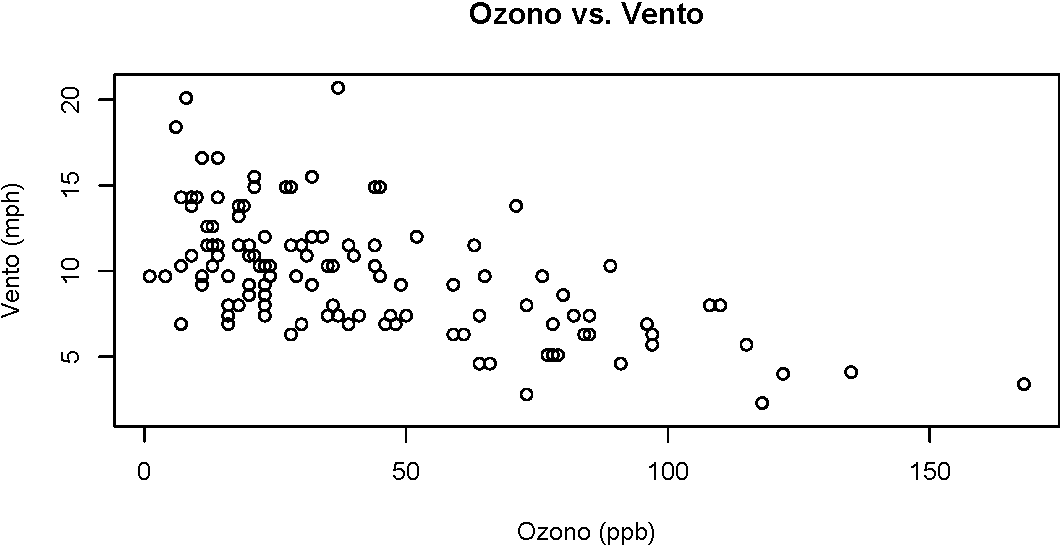
\includegraphics[width=11cm]{o_vs_v}
				\caption{}
				\label{fig:o_vs_v}
			\end{figure}\iftoggle{sol}{\vspace{-2mm}}{~\makeemptybox{1in}}
	
			\begin{solution}
				\begin{rcode}
					plot(airquality$Ozono, airquality$Vento, main="Ozono vs. Vento",
						xlab="Ozono (ppb)", ylab="Vento (mph)")
				\end{rcode}
			\end{solution}
		
%		\iftoggle{sol}{\pagebreak}{}
		
		\part[1\half] Escreva o código necessário para criar um gráfico de barras com a contagem do número de dias em que o arco-íris apareceu e não apareceu, para os dias em que a temperatura foi maior que 90\degree F (\autoref{fig:rainbows}).
		
		\begin{figure}[!htb]
			\centering
			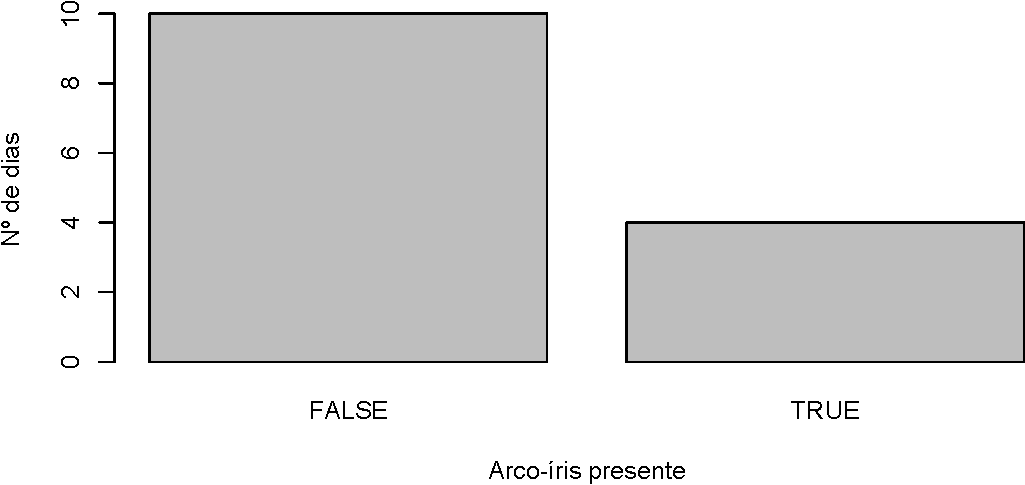
\includegraphics[width=11cm]{rainbows}
			\caption{}
			\label{fig:rainbows}
		\end{figure}\iftoggle{sol}{}{~\makeemptybox{1in}}
		
		\begin{solution}
			\begin{rcode}
				barplot(table(subset(airquality, Temp > 90, ArcoIris)),
					xlab="Arco-íris presente", ylab="Nº de dias")
			\end{rcode}
		\end{solution}
		
	\end{parts}
	
	\question Considere que o \rinline{data.frame CEGI} contém a pauta com as notas dos alunos de CEGI. Atente às seguintes instruções executadas em R.
	
		\begin{rcode}
			> head(CEGI)
			R1aEpoca R2aEpoca SAS1aEpoca SAS2aEpoca
			Ana        12.1     14.4       15.2       11.7
			Pedro       8.2      6.6       12.3        9.9
			Rui        13.3     13.3       13.3       13.3
			Maria      17.2     15.1        8.2       12.2
			Raquel     18.0     19.0       20.0       17.0
			Duarte     10.1      7.1       12.0        8.9
			> str(CEGI)
			'data.frame':	131 obs. of  4 variables:
			$ R1aEpoca  : num  12.1 8.2 13.3 17.2 18 10.1 ...
			$ R2aEpoca  : num  14.4 6.6 13.3 15.1 19 7.1 ...
			$ SAS1aEpoca: num  15.2 12.3 13.3 8.2 20 12 ...
			$ SAS2aEpoca: num  11.7 9.9 13.3 12.2 17 8.9 ...
		\end{rcode}
	
	\begin{parts}
		\part[0\half] Escreva o código necessário para guardar o conteúdo deste \rinline{data.frame} num ficheiro com nome à sua escolha. O ficheiro guardado deve ter um aspecto idêntico ao do seguinte excerto.
		
		\begin{minted}[autogobble]{text}
			R1aEpoca|R2aEpoca|SAS1aEpoca|SAS2aEpoca
			Ana|12,1|14,4|15,2|11,7
			Pedro|8,2|6,6|12,3|9,9
			Rui|13,3|13,3|13,3|13,3
			Maria|17,2|15,1|8,2|12,2
		\end{minted}
		
		\iftoggle{sol}{}{\vspace{-8mm}~\makeemptybox{1in}}
		
		\begin{solution}
			\begin{rcode}
				write.table(CEGI, 'pauta.dat', sep='|', dec=',', quote=FALSE)
			\end{rcode}
		\end{solution}

		\part[1\half] Crie uma função que permita calcular a nota final de cada aluno, sabendo que:
			\begin{itemize}
				\item R1aEpoca e R2aEpoca são as notas dos exames de 1ª e de 2ª épocas de R.
				\item SAS1aEpoca e SAS2aEpoca são as notas dos exames de 1ª e de 2º épocas de SAS.
				\item A nota final é dada pela melhor nota entre a 1ª e a 2ª época.
				\item A nota de cada época é dada pela média entre a nota de R e de SAS.
				\item Caso a nota do exame de R ou de SAS seja inferior a 8 valores o aluno reprova com 8 valores.
			\end{itemize}
			
			Depois de criar a sua função, use-a, para calcular a nota final de todos os alunos.
			
			\begin{solution}
				\begin{minted}[autogobble]{r}
nota_final = function (notas) {
	if (any(notas < 8)) {
		nota = 8
	} else {
		nota = max(mean(notas[1:2]), mean(notas[3:4]))
	}
	return(nota)
}
apply(CEGI, 1, nota_final)
				\end{minted}
			\end{solution}
			
			\iftoggle{sol}{}{~\makeemptybox{2in}}
		
	\end{parts}
	
	\question[2] O vector \rinline{precip} contém a precipitação (chuva) média anual, em polegadas (in), de 70 cidades norte americanas. As seguintes instruções executadas em \textbf{R} fornecem uma noção sobre a estrutura deste objecto.
	
	\begin{rcode}
		> str(precip)
		Named num [1:70] 67 54.7 7 48.5 14 17.2 20.7 13 43.4 40.2 ...
		- attr(*, "names")= chr [1:70] "Mobile" "Juneau" "Phoenix" "Little Rock" ...
		> head(precip)
		Mobile      Juneau     Phoenix Little Rock Los Angeles  Sacramento
		67.0        54.7         7.0        48.5        14.0        17.2
	\end{rcode}
	
	Explique, por palavras suas, o que se pretende encontrar com o seguinte bloco de código, e como isso é conseguido.
	
	\begin{minted}[linenos=true, autogobble]{r}
		cidades = strsplit(names(precip), " ")
		names(precip)[sapply(cidades, function(x) length(x) > 2)]
	\end{minted}
	
	\iftoggle{sol}{}{~\makeemptybox{4in}}
	
	\begin{solution}
		Pretende-se encontrar os nomes das cidades, existentes no vector \rinline{precip}, cujos nomes são compostos por mais de duas palavras.
		
		Na primeira linha, a função \rinline{strsplit} é usada para separar os nomes dos elementos do vector \rinline{precip} por palavras (espaços vazios existentes nos nomes). Esta função separa elementos do tipo caracter, dado um determinado separador, e recebe como argumentos os nomes dos elementos do vector, e o caracter correspondente ao separador, na primeira e na segunda posição, respectivamente. O resultado da utilização desta função é uma lista, guardada numa nova variável denominada \rinline{cidades}, em que cada atributo é um vector com o conjunto de palavras separadas, havendo tantos atributos quanto o comprimento do vector \rinline{precip}.
		
		Na segunda linha, a função \rinline{sapply} é utilizada para percorrer cada atributo da nova lista, aplicando uma função anónima a cada atributo. Esta função devolve um valor lógico, conforme o número de elementos nesse atributo é ou não superior a dois. Este vector lógico resultante é então usado para indexar o vector contendo os nomes do vector \rinline{precip}.
	\end{solution}
	
\end{questions}

\iftoggle{sol}{}{
	\vspace{10mm}
	\begin{center}
		\gradetable[h][questions]
		\small{\\ \vspace{3mm}(a preencher pelo docente)}
	\end{center}
}
	
\end{document}